\documentclass[11pt,preprint]{elsarticle}

\usepackage{lmodern}
%%%% My spacing
\usepackage{setspace}
\setstretch{1.2}
\DeclareMathSizes{12}{14}{10}{10}

% Wrap around which gives all figures included the [H] command, or places it "here". This can be tedious to code in Rmarkdown.
\usepackage{float}
\let\origfigure\figure
\let\endorigfigure\endfigure
\renewenvironment{figure}[1][2] {
    \expandafter\origfigure\expandafter[H]
} {
    \endorigfigure
}

\let\origtable\table
\let\endorigtable\endtable
\renewenvironment{table}[1][2] {
    \expandafter\origtable\expandafter[H]
} {
    \endorigtable
}


\usepackage{ifxetex,ifluatex}
\usepackage{fixltx2e} % provides \textsubscript
\ifnum 0\ifxetex 1\fi\ifluatex 1\fi=0 % if pdftex
  \usepackage[T1]{fontenc}
  \usepackage[utf8]{inputenc}
\else % if luatex or xelatex
  \ifxetex
    \usepackage{mathspec}
    \usepackage{xltxtra,xunicode}
  \else
    \usepackage{fontspec}
  \fi
  \defaultfontfeatures{Mapping=tex-text,Scale=MatchLowercase}
  \newcommand{\euro}{€}
\fi

\usepackage{amssymb, amsmath, amsthm, amsfonts}

\def\bibsection{\section*{References}} %%% Make "References" appear before bibliography


\usepackage[numbers]{natbib}

\usepackage{longtable}
\usepackage[margin=2.3cm,bottom=2cm,top=2.5cm, includefoot]{geometry}
\usepackage{fancyhdr}
\usepackage[bottom, hang, flushmargin]{footmisc}
\usepackage{graphicx}
\numberwithin{equation}{section}
\numberwithin{figure}{section}
\numberwithin{table}{section}
\setlength{\parindent}{0cm}
\setlength{\parskip}{1.3ex plus 0.5ex minus 0.3ex}
\usepackage{textcomp}
\renewcommand{\headrulewidth}{0.2pt}
\renewcommand{\footrulewidth}{0.3pt}

\usepackage{array}
\newcolumntype{x}[1]{>{\centering\arraybackslash\hspace{0pt}}p{#1}}

%%%%  Remove the "preprint submitted to" part. Don't worry about this either, it just looks better without it:
\makeatletter
\def\ps@pprintTitle{%
  \let\@oddhead\@empty
  \let\@evenhead\@empty
  \let\@oddfoot\@empty
  \let\@evenfoot\@oddfoot
}
\makeatother

 \def\tightlist{} % This allows for subbullets!

\usepackage{hyperref}
\hypersetup{breaklinks=true,
            bookmarks=true,
            colorlinks=true,
            citecolor=blue,
            urlcolor=blue,
            linkcolor=blue,
            pdfborder={0 0 0}}


% The following packages allow huxtable to work:
\usepackage{siunitx}
\usepackage{multirow}
\usepackage{hhline}
\usepackage{calc}
\usepackage{tabularx}
\usepackage{booktabs}
\usepackage{caption}


\newenvironment{columns}[1][]{}{}

\newenvironment{column}[1]{\begin{minipage}{#1}\ignorespaces}{%
\end{minipage}
\ifhmode\unskip\fi
\aftergroup\useignorespacesandallpars}

\def\useignorespacesandallpars#1\ignorespaces\fi{%
#1\fi\ignorespacesandallpars}

\makeatletter
\def\ignorespacesandallpars{%
  \@ifnextchar\par
    {\expandafter\ignorespacesandallpars\@gobble}%
    {}%
}
\makeatother


% definitions for citeproc citations
\NewDocumentCommand\citeproctext{}{}
\NewDocumentCommand\citeproc{mm}{%
\href{\#cite.\detokenize{#1}}{#2}\nocite{#1}}

\makeatletter
% allow citations to break across lines
\let\@cite@ofmt\@firstofone
% avoid brackets around text for \cite:
\def\@biblabel#1{}
\def\@cite#1#2{{#1\if@tempswa , #2\fi}}
\makeatother
\newlength{\cslhangindent}
\setlength{\cslhangindent}{1.5em}
\newlength{\csllabelwidth}
\setlength{\csllabelwidth}{3em}
\newenvironment{CSLReferences}[2] % #1 hanging-indent, #2 entry-spacing
{\begin{list}{}{%
	\setlength{\itemindent}{0pt}
	\setlength{\leftmargin}{0pt}
	\setlength{\parsep}{0pt}
	% turn on hanging indent if param 1 is 1
	\ifodd #1
	\setlength{\leftmargin}{\cslhangindent}
	\setlength{\itemindent}{-1\cslhangindent}
	\fi
	% set entry spacing
	\setlength{\itemsep}{#2\baselineskip}}}
{\end{list}}

\usepackage{calc}
\newcommand{\CSLBlock}[1]{\hfill\break\parbox[t]{\linewidth}{\strut\ignorespaces#1\strut}}
\newcommand{\CSLLeftMargin}[1]{\parbox[t]{\csllabelwidth}{\strut#1\strut}}
\newcommand{\CSLRightInline}[1]{\parbox[t]{\linewidth - \csllabelwidth}{\strut#1\strut}}
\newcommand{\CSLIndent}[1]{\hspace{\cslhangindent}#1}


\urlstyle{same}  % don't use monospace font for urls
\setlength{\parindent}{0pt}
\setlength{\parskip}{6pt plus 2pt minus 1pt}
\setlength{\emergencystretch}{3em}  % prevent overfull lines
\setcounter{secnumdepth}{5}

%%% Use protect on footnotes to avoid problems with footnotes in titles
\let\rmarkdownfootnote\footnote%
\def\footnote{\protect\rmarkdownfootnote}
\IfFileExists{upquote.sty}{\usepackage{upquote}}{}

%%% Include extra packages specified by user
\providecommand{\pandocbounded}[1]{#1}

%%% Hard setting column skips for reports - this ensures greater consistency and control over the length settings in the document.
%% page layout
%% paragraphs
\setlength{\baselineskip}{12pt plus 0pt minus 0pt}
\setlength{\parskip}{12pt plus 0pt minus 0pt}
\setlength{\parindent}{0pt plus 0pt minus 0pt}
%% floats
\setlength{\floatsep}{12pt plus 0 pt minus 0pt}
\setlength{\textfloatsep}{20pt plus 0pt minus 0pt}
\setlength{\intextsep}{14pt plus 0pt minus 0pt}
\setlength{\dbltextfloatsep}{20pt plus 0pt minus 0pt}
\setlength{\dblfloatsep}{14pt plus 0pt minus 0pt}
%% maths
\setlength{\abovedisplayskip}{12pt plus 0pt minus 0pt}
\setlength{\belowdisplayskip}{12pt plus 0pt minus 0pt}
%% lists
\setlength{\topsep}{10pt plus 0pt minus 0pt}
\setlength{\partopsep}{3pt plus 0pt minus 0pt}
\setlength{\itemsep}{5pt plus 0pt minus 0pt}
\setlength{\labelsep}{8mm plus 0mm minus 0mm}
\setlength{\parsep}{\the\parskip}
\setlength{\listparindent}{\the\parindent}
%% verbatim
\setlength{\fboxsep}{5pt plus 0pt minus 0pt}



\begin{document}



\begin{frontmatter}  %

\title{Simple Beats Clever: Building a Constrained Global Balanced Index
Fund}

% Set to FALSE if wanting to remove title (for submission)




\author[Add1]{Kieron Maseko (26572982)}
\ead{26572982@sun.ac.za}





\address[Add1]{Stellenbosch University, Stellenbosch, South Africa}

\cortext[cor]{Corresponding author: Kieron Maseko (26572982)}

\begin{abstract}
\small{
This report builds a global balanced index fund for a local investor
under a strict mandate: long-only, quarterly rebalancing, at most 25\%
in bonds, 75\% in equities, 15\% in commodities, 60\% offshore and 35\%
in any single asset, using only assets with at least five years of data.
Using monthly returns since 2010 on global and local equities, bonds and
commodities, we compare a minimum-volatility portfolio, a mean-variance
portfolio and a static balanced mix from 2020 to 2026. All three meet
the mandate at every rebalance. The optimised portfolios did not beat
the simple static mix: it had the highest Sharpe ratio, while the
mean-variance portfolio, concentrated in a few past winners, suffered
the deepest drawdown. Whatever the method, equities drive more than 80\%
of portfolio risk.
}
\end{abstract}

\vspace{1cm}


\begin{keyword}
\footnotesize{
Portfolio Optimisation \sep Minimum Variance \sep Mean-Variance
\sep Risk Contribution \sep Multi-Asset \\
\vspace{0.3cm}
}
\footnotesize{
\textit{JEL classification} G11 \sep G15
}
\end{keyword}



\vspace{0.5cm}

\end{frontmatter}

\setcounter{footnote}{0}



%________________________
% Header and Footers
%%%%%%%%%%%%%%%%%%%%%%%%%%%%%%%%%
\pagestyle{fancy}
\chead{}
\rhead{}
\lfoot{}
\rfoot{\footnotesize Page \thepage}
\lhead{}
%\rfoot{\footnotesize Page \thepage } % "e.g. Page 2"
\cfoot{}

%\setlength\headheight{30pt}
%%%%%%%%%%%%%%%%%%%%%%%%%%%%%%%%%
%________________________

\headsep 35pt % So that header does not go over title




\section{\texorpdfstring{Introduction
\label{Introduction}}{Introduction }}\label{introduction}

A global balanced fund has to do two things at once: spread risk across
regions and asset classes, and stay inside a mandate. This report builds
such a fund for a local investor. The mandate is long-only, rebalanced
quarterly, with at most 25\% in bonds and credit, 75\% in equities, 15\%
in commodities, 60\% offshore and 35\% in any single asset. Assets need
at least five years of data, and the covariance matrix is estimated on
monthly data from 2010.

We compare three ways of setting the weights: a minimum-volatility
(MinVol) portfolio, a mean-variance (MeanVar) portfolio
(\citeproc{ref-markowitz1952}{Markowitz, 1952}), and a static balanced
mix that does not use the data at all. The short answer is that the
optimisers did not beat the simple mix, and that, whatever the method,
equities carry most of the risk.

\section{\texorpdfstring{Data and Methodology
\label{Data}}{Data and Methodology }}\label{data-and-methodology}

The universe has 17 assets (Table \ref{tab:assets}): four MSCI equity
regions, three 10-year government bonds (US, Germany and UK), the
Bloomberg Commodity index and gold offshore; and locally the Top 40
(Large Caps), Mid Caps, three factor indexes (Momentum, Value and Low
Volatility), Listed Property, the ALBI and inflation-linked bonds.
Listed Property is classed as equity. All returns are monthly, from
January 2010 to September 2026.

The global bond files contain yields, not prices, so we build a total
return index from them. Each month's return is the carry minus the price
effect of the yield change: \[
r_t \approx \frac{y_{t-1}}{12} - D_{t-1}\,\Delta y_t, \qquad D = \frac{1-(1+y)^{-10}}{y},
\] where \(D\) is the (modified) duration of a 10-year bond. This
approximation captures the 2022 bond crash: the German, UK and US
proxies lost about 23\%, 21\% and 17\% that year.

\begin{table}[H]
\centering
\caption{Asset universe: annualised return and volatility over each asset's full sample \label{tab:assets}} 
\begingroup\footnotesize
\begin{tabular}{llllrrr}
  \hline
Name & Class & Region & Start & Months & Return (\%) & Vol (\%) \\ 
  \hline
Germany 10Yr & Bonds & Global & 2010-01 & 201 & 0.8 & 6.7 \\ 
  UK 10Yr & Bonds & Global & 2010-01 & 201 & 1.2 & 7.7 \\ 
  US 10Yr & Bonds & Global & 2010-01 & 201 & 1.6 & 7.2 \\ 
  Bcom Index & Commodity & Global & 2010-01 & 201 & 0.1 & 14.8 \\ 
  Gold & Commodity & Global & 2010-01 & 201 & 8.3 & 16.5 \\ 
  MSCI EM & Equity & Global & 2010-01 & 201 & 6.1 & 17.9 \\ 
  MSCI EU & Equity & Global & 2010-01 & 201 & 7.5 & 16.9 \\ 
  MSCI Jap & Equity & Global & 2010-01 & 201 & 8.4 & 14.2 \\ 
  MSCI USA & Equity & Global & 2010-01 & 201 & 14.3 & 14.5 \\ 
  SA Bonds & Bonds & Local & 2010-01 & 201 & 9.7 & 7.7 \\ 
  SA ILB & Bonds & Local & 2010-01 & 201 & 7.7 & 6.1 \\ 
  SA Large & Equity & Local & 2015-01 & 141 & 10.9 & 15.1 \\ 
  SA LowVol & Equity & Local & 2024-01 & 33 & 13.5 & 11.4 \\ 
  SA Mid & Equity & Local & 2015-01 & 141 & 7.3 & 15.9 \\ 
  SA Momentum & Equity & Local & 2017-04 & 114 & 10.0 & 15.9 \\ 
  SA Property & Equity & Local & 2010-01 & 201 & 9.9 & 18.8 \\ 
  SA Value & Equity & Local & 2018-04 & 102 & 10.9 & 16.5 \\ 
   \hline
\end{tabular}
\endgroup
\end{table}

At each quarter-end from December 2019 we estimate the mean vector
\(\mu\) (geometric mean) and the covariance matrix \(\Sigma\) on an
expanding window from 2010, so the look-back is always at least ten
years. Assets with fewer than 60 months of data are excluded; as a
result Low Volatility never enters, Momentum enters in 2022 and Value in
2023. Because local data start later, \(\Sigma\) is estimated on
pairwise-complete data and adjusted to the nearest positive definite
matrix. The two optimised portfolios solve

\[
\text{MinVol:}\; \min_w\, w'\Sigma w \qquad\qquad \text{MeanVar:}\; \max_w\, w'\mu - \frac{\lambda}{2}\, w'\Sigma w, \quad \lambda = 4,
\] subject to \(\sum_i w_i = 1\), \(0 \le w_i \le 0.35\), and the class
and regional caps above. The static mix holds 60\% equity, 25\% bonds
and 15\% commodities, with 50\% offshore. Weights are applied from the
month after each rebalance, and drift with returns in between.

\section{\texorpdfstring{Results
\label{Results}}{Results }}\label{results}

\subsection{Meeting the mandate}\label{meeting-the-mandate}

Table \ref{tab:limits} shows the largest exposure each portfolio took at
any rebalance date. All limits are met. The optimisers push straight to
the binding constraints: MinVol fills the bond, commodity and offshore
caps, because these assets lower volatility, while MeanVar fills the
single-asset cap and holds only a handful of assets.

\begin{table}[H]
\centering
\caption{Largest exposure at any rebalance date (limits: 0.35, 0.25, 0.75, 0.15, 0.60) \label{tab:limits}} 
\begingroup\footnotesize
\begin{tabular}{lrrrrrr}
  \hline
Portfolio & Max single & Bonds & Equity & Commodity & Global & Max assets \\ 
  \hline
Min Volatility & 0.33 & 0.25 & 0.60 & 0.15 & 0.60 &  10 \\ 
  Mean-Variance & 0.35 & 0.25 & 0.75 & 0.15 & 0.60 &   5 \\ 
  Static Balanced & 0.20 & 0.25 & 0.60 & 0.15 & 0.50 &  14 \\ 
   \hline
\end{tabular}
\endgroup
\end{table}

Figure \ref{fig:weights} shows how the weights moved. MinVol stays well
spread, with a large offshore bond and commodity block. MeanVar is much
more concentrated: at the latest rebalance it holds only 4 assets, led
by US equities at the 35\% cap, local Large Caps and the ALBI.

\begin{figure}
\centering
\pandocbounded{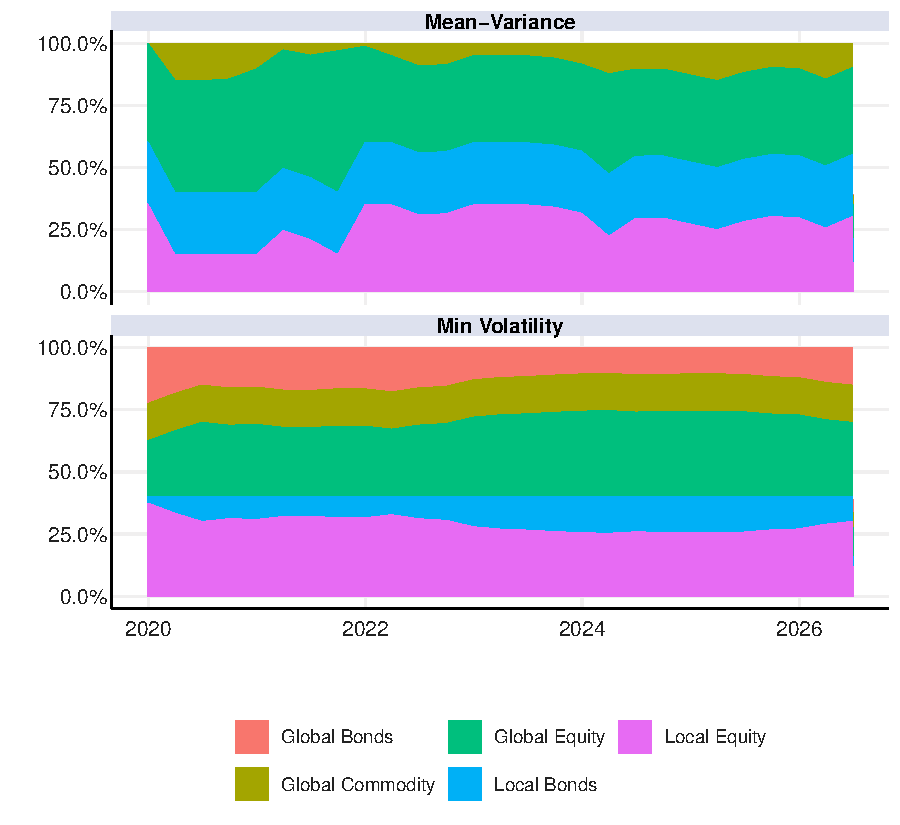
\includegraphics[keepaspectratio,alt={Portfolio weights by region and asset class at each rebalance }]{Question4_files/figure-latex/weights-1.pdf}}
\caption{Portfolio weights by region and asset class at each rebalance
\label{fig:weights}}
\end{figure}

\subsection{Performance}\label{performance}

Table \ref{tab:perf} and Figure \ref{fig:cum} compare the three
portfolios from January 2020. The static mix had the best return and the
best Sharpe ratio, at almost the same volatility as MinVol. MeanVar was
the worst on every risk measure: its drawdown of 26.7\% was much deeper
than the others, because it bet on the few assets with the best history.
This is the well-known estimation-error problem: optimisers treat noisy
historical means as if they were known, and simple mixes are hard to
beat out of sample (\citeproc{ref-demiguel2009}{DeMiguel, Garlappi \&
Uppal, 2009}).

\begin{table}[H]
\centering
\caption{Backtest performance, January 2020 to September 2026 (monthly returns) \label{tab:perf}} 
\begingroup\footnotesize
\begin{tabular}{llll}
  \hline
Measure & Min Volatility & Mean-Variance & Static Balanced \\ 
  \hline
Annualised return & 10.0\% & 10.7\% & 11.3\% \\ 
  Annualised volatility & 11.5\% & 13.9\% & 11.4\% \\ 
  Sharpe ratio & 0.87 & 0.77 & 0.99 \\ 
  Maximum drawdown & 15.8\% & 26.7\% & 16.9\% \\ 
  Modified ES (95\%) & -7.7\% & -14.0\% & -7.8\% \\ 
   \hline
\end{tabular}
\endgroup
\end{table}

\begin{figure}
\centering
\pandocbounded{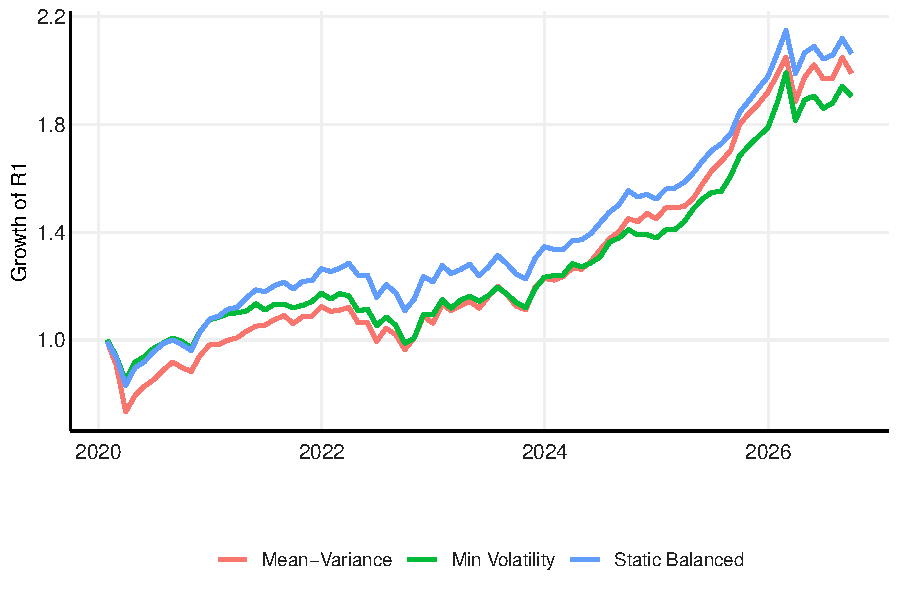
\includegraphics[keepaspectratio,alt={Cumulative return of the three portfolios }]{Question4_files/figure-latex/cum-1.pdf}}
\caption{Cumulative return of the three portfolios \label{fig:cum}}
\end{figure}

\subsection{Where the risk comes from}\label{where-the-risk-comes-from}

Weights can be misleading. The share of portfolio variance from asset
\(i\) is \[
RC_i = \frac{w_i\,(\Sigma w)_i}{w'\Sigma w}, \qquad \sum_i RC_i = 1 .
\] Table \ref{tab:risk} shows that at the latest rebalance equities make
up 60--65\% of each portfolio but more than 80\% of its risk, while
bonds carry 25\% of the weight but only 5--12\% of the risk. A
``balanced'' fund is, in risk terms, still mainly an equity fund. An
equal-risk-contribution portfolio would spread risk more evenly
(\citeproc{ref-maillard2010}{Maillard, Roncalli \& Teiletche, 2010}).

\begin{table}[H]
\centering
\caption{Weight / share of risk by asset class at the June 2026 rebalance \label{tab:risk}} 
\begingroup\footnotesize
\begin{tabular}{llll}
  \hline
Portfolio & Bonds & Commodity & Equity \\ 
  \hline
Min Volatility & 25\% / 6\% & 15\% / 12\% & 60\% / 82\% \\ 
  Mean-Variance & 25\% / 12\% & 10\% / 6\% & 65\% / 82\% \\ 
  Static Balanced & 25\% / 9\% & 15\% / 12\% & 60\% / 80\% \\ 
   \hline
\end{tabular}
\endgroup
\end{table}

\subsection{Practical points}\label{practical-points}

Two practical issues matter for running the fund. First, the limits only
hold at rebalance dates. Between rebalances, MinVol's offshore weight
drifted up to 62.6\% and its largest position to 35.3\%, above the 60\%
and 35\% caps. In practice the fund should target slightly below each
cap, or rebalance early when a cap is breached. Second, costs are low:
average one-way turnover is 7.0\% per quarter for MinVol and 5.2\% for
MeanVar, because the expanding window changes slowly.

\section{\texorpdfstring{Conclusion
\label{Conclusion}}{Conclusion }}\label{conclusion}

All three portfolios meet the mandate, but the simplest one did best.
The static 60/25/15 mix had the highest Sharpe ratio, the
minimum-volatility portfolio matched its risk without beating its
return, and the mean-variance portfolio was concentrated and fragile. We
would therefore recommend a static or minimum-volatility core, with
weights set slightly inside the limits to allow for drift. The results
have limits: global assets are in US dollars and local assets in rand,
with no currency conversion; the global bond returns are a duration
approximation; and the local series are short, so the covariance matrix
leans heavily on global data. Shrinking the covariance matrix, or
targeting equal risk contributions, are natural next steps.

\newpage

\section*{References}\label{references}
\addcontentsline{toc}{section}{References}

\protect\phantomsection\label{refs}
\begin{CSLReferences}{1}{1}
\bibitem[\citeproctext]{ref-demiguel2009}
DeMiguel, V., Garlappi, L. \& Uppal, R. 2009. Optimal versus naive
diversification: How inefficient is the 1/n portfolio strategy?
\emph{The Review of Financial Studies}. 22(5):1915--1953.

\bibitem[\citeproctext]{ref-maillard2010}
Maillard, S., Roncalli, T. \& Teiletche, J. 2010. The properties of
equally weighted risk contribution portfolios. \emph{The Journal of
Portfolio Management}. 36(4):60--70.

\bibitem[\citeproctext]{ref-markowitz1952}
Markowitz, H. 1952. Portfolio selection. \emph{The Journal of Finance}.
7(1):77--91.

\end{CSLReferences}

\bibliography{Tex/ref}





\end{document}
